\documentclass[Report.tex]{subfiles}

\begin{document}

\begin{figure}
\center
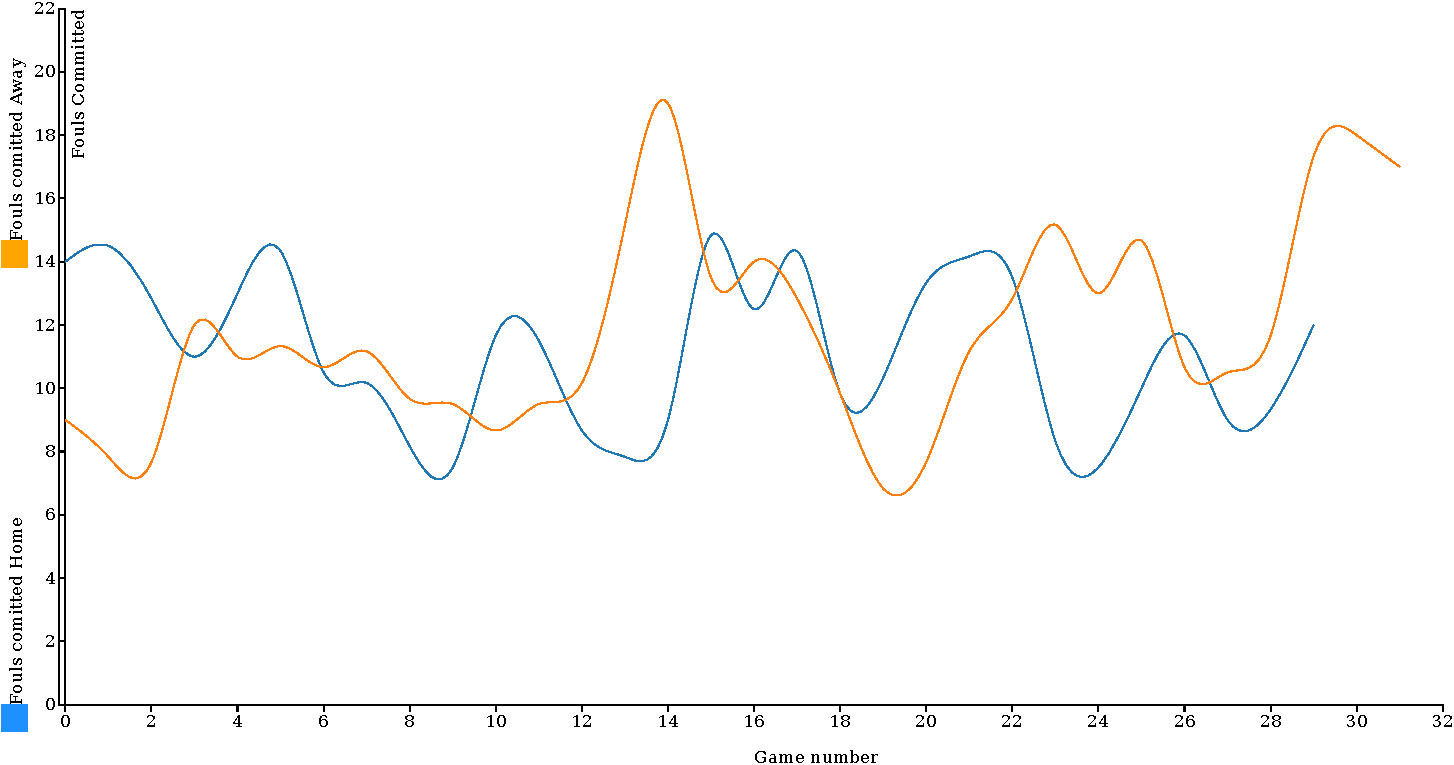
\includegraphics[width=\textwidth]{Figures/fouls.pdf}
\caption{A line chart showing fouls committed throughout a season, split up in those committed home, and those away.}
\label{Fig:FOULS}
\end{figure}


\subsubsection{What-why-how}
Figure \ref{Fig:FOULS} is the result of Exploratory Data Analysis. The hypothesis behind it, was that the closer to the end of a season, teams would get more aggressive. The idea behind splitting home and away matches up, is that a team might be more comfortable when playing home than away, which could influence the results.\\
The idea was to plot the fouls committed throughout a season and see some sort of trend, one of the things line charts are especially useful for. However, it turned out that no apparent trend could be found from the data available. However, what could be seen, is that the spikes of fouls committed is consistently higher when away. One thing to mention, is that in the dataset plotted, the season is not complete yet, as seen on the chart, a few matches are missing on the home variable.

\subsubsection{Code}
The code behind this chart lies in gathering and processing statistics for a team over multiple rounds, then filtering it for everything else than the foul statistics, while still preserving the right order of the matches. After that is done, it is put in D3, with some relatively simple code for a line chart.

\end{document}
